\begin{center}
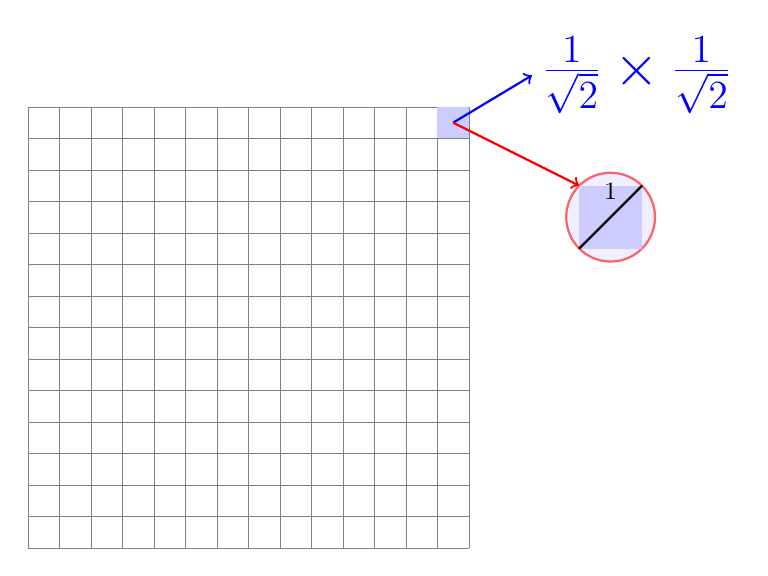
\begin{tikzpicture}[scale=0.4]
    % Draw 14x14 grid
    \draw[step=1cm,gray,very thin] (0,0) grid (14,14);
    
    % Highlight the top-right square in blue
    \fill[blue!20] (13,13) rectangle (14,14);

    \draw[blue, ->, thick] (13.5, 13.5) -- (16, 15) node[right] {\textbf{\textit{\huge $\frac{1}{\sqrt{2}} \times \frac{1}{\sqrt{2}}$}}};

    % Arrow pointing 45 degrees down-right, ending at the circumference of the circle
    

    % Draw the circumscribed circle
    \draw[red, thick, fill=blue!10, opacity=0.6] (18.5, 10.5) circle (1.41cm);

    % Large square inside the circle
    \fill[blue!20] (17.5,9.5) rectangle (19.5,11.5);

    % Label the diameter of the circle as 1
    \draw[thick] (17.5, 9.5) -- (19.5, 11.5); % Diameter line
    \node at (18.5, 11.3) {\small $1$}; % Label for the diameter

    \draw[red, ->, thick] (13.5, 13.5) -- (17.5, 11.5);
\end{tikzpicture}
\end{center}